\newgeometry{top=2cm, bottom=1.8cm, left=3.3cm, right=3.5cm} 
\setlength{\columnsep}{1cm}

\begin{multicols*}{2}



\begin{center}
\begin{tabular}{|c|c|c|}
\hline
\textbf{a} & 0 & a \\ \hline
\textbf{b} & 0 & b \\ \hline
\textbf{c} & 0 & c \\ \hline
\textbf{d} & 1 & cdj \\ \hline
\textbf{e} & 1 & abi \\ \hline
\textbf{f} & 1 & fgl \\ \hline
\textbf{g} & 0 & g \\ \hline
\textbf{k} & 2 & abicdjk \\ \hline
\textbf{l} & 2 & fg \\ \hline
\textbf{m} & 2 & abicdjfglm \\ \hline
\textbf{h} & 0 & h \\ \hline
\textbf{L} & 2 & abicdjfglmhL \\ \hline
\end{tabular}
\end{center}
\begin{center}
    \textbf{Рис. 8.}
\end{center}


\begin{center}
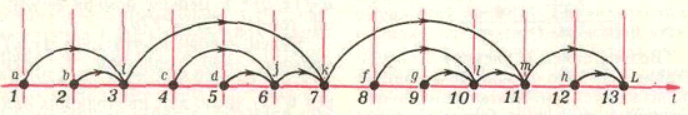
\includegraphics[width=1\textwidth]{png9.png} \\
\textbf{Рис. 9.}
\end{center}

Один из алгоритмов построения таких укладок, известный под названием \textit{алгоритма Реджеевского}, мы сейчас опишем

\vspace{0.3cm}
\noindent\textbf{Шаг 1.} Построим таблицу с $n$ строками и тремя столбцами, где $n$ — число вершин ордера.

\vspace{0.3cm}
\noindent\textbf{Шаг 2.} Заполним первый столбец таблицы снизу вверх, поместив в самой нижней строке корень $x_0$ ордера, затем в произвольном порядке его предшественников, лишь бы нигде не нарушалась очередность вычислений. (то есть любые данные, нужные для очередной операции, должны быть получены раньше её выполнения)

Далее через p(x) и q(x) мы будем обозначать записи во втором и третьем столбцах строки, начинающейся с буквы x. Значениями функции p будут числа, функции q - последовательности букв. Пусть уже заполнены первые r строк

\vspace{0.3cm}
\noindent\textbf{Шаг 3.} Приступаем к заполнению очередной строки (предыдущие уже заполнены); Обозначим через x ее первую букву. Если вершина x - висячая, переходим к шагу 4, в противном случае - к шагу 5.

\vspace{0.3cm}
\noindent\textbf{Шаг 4.} Во втором столбце пишем 0, в третьем — $x$. (Таким образом, мы положили p(x) = 0, q(x) = x) Переходим к шагу 3.

\vspace{5cm}
\noindent\textbf{Шаг 5.} Пусть $y_1, y_2, \dots, y_k$ — вершины ордерева, непосредственно предшествующие x, упорядоченные так, что: p(y_1) \geq p(y_2) \geq \dots \geq (y_k). \text{Найдём}:

\begin{align}
p(x) &= \max \{ p(y_s) + t_s \}, \\
q(x) &= q(y_1) q(y_2) \dots q(y_k).
\end{align}
и внесем найденные значения во второй и третий столбцы, рассматриваемой строки. Переходим к шагу 3.

\vspace{7cm}
\noindent Повторяем шаги 3–5, пока не будет заполнена вся таблица. Тогда в последней строке во втором столбце мы получим ширину укладки, то есть $p(x_0) = W(y, T)$, а в третьем саму - укладку дерева T, если вершины в последовательности $q(x_0)$ занумеровать слева направо.

Таблица, полученная при применении алгоритма Реджеевского к ордереву на рисунке 7, показана на рисунке 8, а «уложенное» ордерево - на рисунке 9.

\end{multicols*}
